\documentclass[12pt]{article}
\usepackage[utf8]{inputenc}
\usepackage[russian]{babel}
\usepackage{graphicx}
\usepackage[none]{hyphenat}
\graphicspath{ {pictures} }
\begin{document}
{\Large\textbf {Отчёт по второму заданию курса "Численное моделирование реагирующих потоков"}\par}
\textit{Выполнил студент 031 группы Александр Казаков}

\section{Численный метод}
Для решения системы ОДУ $\frac{d\vec{y}}{dt} = \vec{f}({\vec{y}, t)$ используется неявный метод Эйлера первого порядка точности, также известный как метод Гира первого порядка.
\begin{eqnarray}
\frac{\vec{y_{n+1}} - \vec{y_n}}{\tau} = \vec{f}(\vec{y_{n+1}}, t) + o(\tau)
\end{eqnarray}
Для решения возникающей системы нелинейных алгебраических уравнений  $\vec{f}(\vec{u}) = 0$ используется метод Ньютона из первого задания. 
На каждой итерации метода искомое решение $\vec{u_k}$ получает приращение $\Delta\vec{u_k}$, рассчитанное из условия:
\begin{eqnarray}
\vec{u_{k+1}} \approx \vec{u_k} + \frac{\partial{\vec{f}}}{\partial{\vec{u}}}\Delta\vec{u_k} = 0
\end{eqnarray}
Для решения полученной СЛАУ использовалась библиотека gsl.
В данном случае рассчитанное значение приращения брать меньшим в два раза не обязательно, метод сходится и без этого.
Было проведено обезразмеривание величин из условия 
\begin{eqnarray}
p' = p/10^6, Q' = Q/10^6, T' = T/10^3, \rho' = \rho,
\end{eqnarray}
что позволило добиться сходимости метода.

\section{Начальные условия}\label{initAppr}
В качестве начальных условий при $x = 0$ выбираются параметры фон Неймана, посчитанные при условии $p_0 = 10^5Pa$ и $T_0 = 293K$:
\begin{eqnarray}
\rho(0) = 9.29 kg/m^3, u(0) = 0.217 km/s, p(0) = 3.33 MPa, Z(0) = 1, T = 1165 K
\end{eqnarray}

\section{Сходимость}\label{converg}
При уменьшении шага по времени на графике решения визуально наблюдается сходимость.

\section{Результаты}\label{results}
Интегрирование проводилось до момента, когда метод Ньютона терял устойчивость из-за приближения $u$ к $c$, то есть знаменателя в одном из уравнений системы к нулю. Это соответствует $x = 25.6 mm$. Значение параметров в этой точке:
\begin{eqnarray}
\rho(0) = 1.99 kg/m^3, u(0) = 1.02 km/s, p(0) = 1.72 MPa, Z(0) = 0.00, T = 2814 K
\end{eqnarray}

\begin{figure}[H]
\center{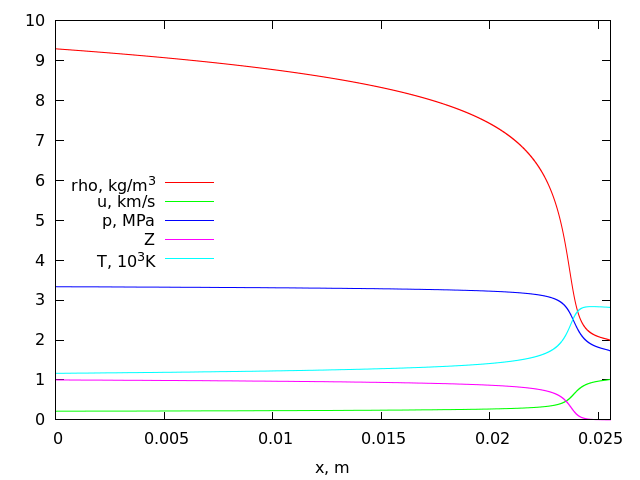
\includegraphics[width=1\linewidth]{pictures/ZeldovichPRho}}
\caption{График полученного решения}
\label{zeldovich}
\end{figure}
\begin{figure}[H]
\center{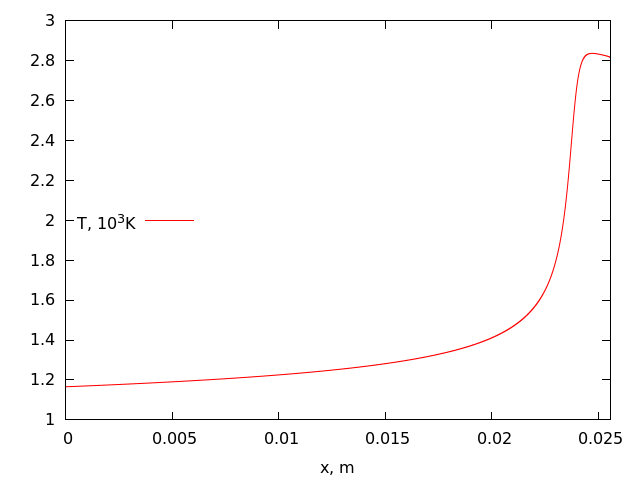
\includegraphics[width=1\linewidth]{pictures/ZeldovichT}}
\caption{График полученного решения подробнее для $T$}
\label{zeldovicht}
\end{figure}
\begin{figure}[H]
\center{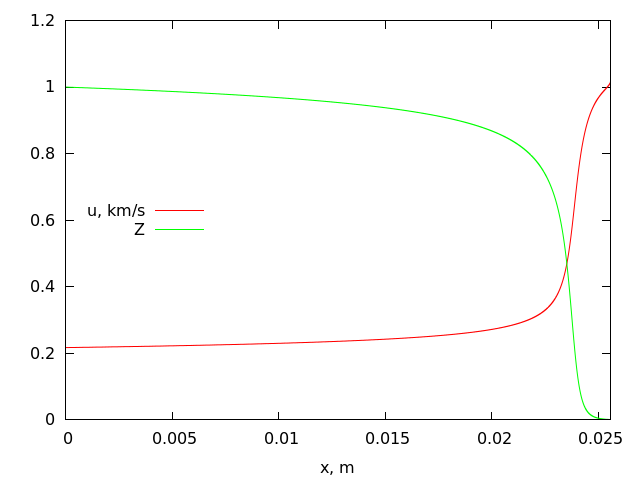
\includegraphics[width=1\linewidth]{pictures/ZeldovichUZ}}
\caption{График полученного решения подробнее для $u$ и $Z$}
\label{zeldovichuz}
\end{figure}

\end{document}
